\chapter{公平性}
\label{chap:trust-fairness}

设想一个分配培训名额的模型：总体上它的预测相当准确，但把它对不同人群的决定拆开看，可能发现某个群体的合格申请者被集中拒绝。要判断这是不是问题，有两件事必须先做：一是看错误落在谁身上、造成什么后果；二是在评价之前确定名额本应按什么原则分配——按现有资格、按培训的预期收益，还是为了弥补机会不足。同一个模型，在不同分配原则下可能得出完全不同的公平结论。即使两个群体的总体准确率相同，误拒合格者与误收不合格者的比例、实际得到的机会数量以及错误造成的损失仍可能差别很大，“准确率一样”说明不了公平。

前两章回答的是“模型错多少、在变化条件下是否仍然可靠”，但准确和稳定并不回答“机会与负担在不同人之间应当怎样分配”：一个模型可以既准确又鲁棒，同时系统性地少给某群人机会。因此公平性是在可靠性证据之上另行提出的规范要求。在第~\ref{chap:trust-foundations}章的三层框架中，它处在要求层：先确定比较哪些待遇、哪些错误和哪些影响路径；群体统计、个体成对对照、因果分析和生成内容评价提供证据；群体构成、标签产生方式和长期后果随时间改变时，还要有监测、复查和纠正。

本章以培训名额分配为主线，回答三个前后相连的问题。第~\ref{sec:fairness-concepts}节先确定要保护谁、保护什么后果，以及不公平从哪些环节产生；没有这一步，后面的指标就没有明确的比较对象。第~\ref{sec:fairness-criteria}节把保护对象写成可检验的准则，并说明准则之间为什么会冲突、有限样本能支持什么结论。第~\ref{sec:fairness-intervention}节按形成原因决定在数据、训练或决策流程中改哪里，再用即时效果和长期反馈检验措施是否改善了后果，而不只是改善了某个统计数字。

图~\ref{fig:trust-fairness-opportunity}用一个构造情景说明个体层面的比较：两名申请者的三项认可资格完全相同，系统却选中一人、拒绝一人。这个教学设定假定三个资格项已经覆盖了名额分配的全部依据，且没有被允许的抽签机制；在这种条件下，无关差异若稳定地带来不同待遇，就违背了该场景的个体一致性。现实审计不能直接照搬：须先验证资格项确实充分、是否存在合法随机机制，“两份材料看起来差不多”本身不足以构成不公平的证据。

\begin{figure*}[!htb]
  \centering
  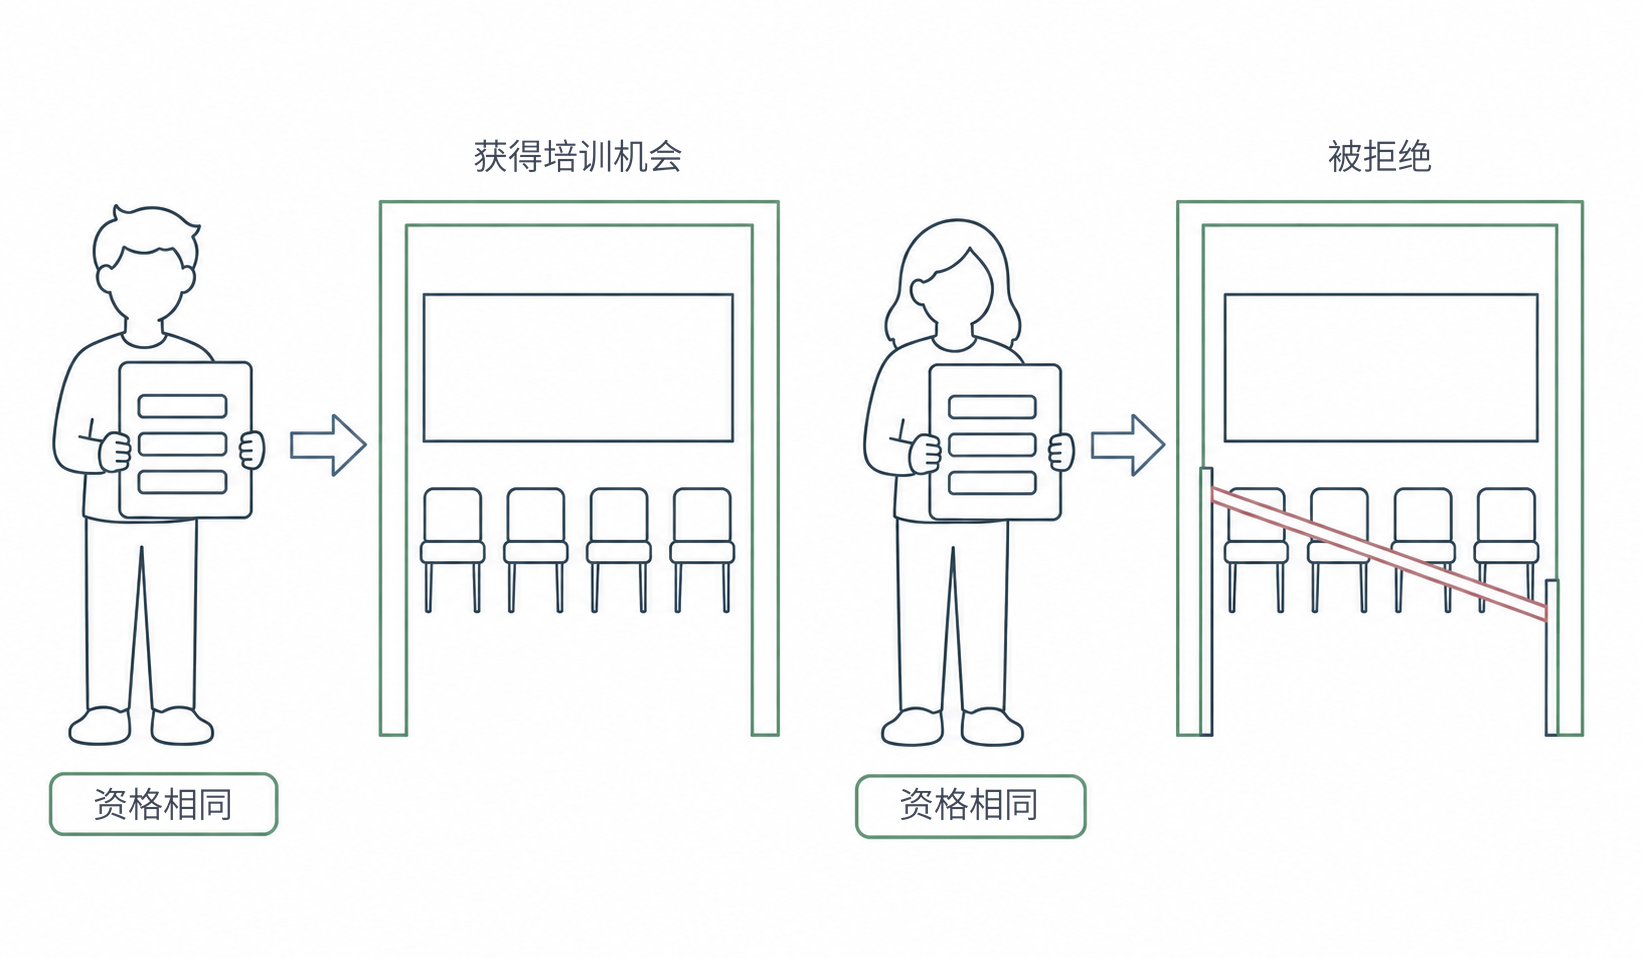
\includegraphics[width=132.000mm]{figures/03-foundations/03-trustworthiness/generated/fairness-opportunity/figure.png}
  \caption{同一系统处理两个认可资格相同的申请者，材料上的三个相同资格项覆盖教学设定的分配依据，一人获选、一人被拒，提示调查个体差别。人物外观只区别对象，未指定差异原因。图为构造情景。}
  \label{fig:trust-fairness-opportunity}
\end{figure*}

\section{模型的公平性}
\label{sec:fairness-concepts}

\subsection{公平性的含义}
\label{sec:fairness-meaning}

开篇的例子已经表明，仅比较准确率无法判断名额分配是否恰当，我们需要一个专门评价“分配”的概念。\term{公平性}（fairness）指依据任务所认可的原则，评价模型及其所在流程怎样在不同人之间分配机会、收益、错误和负担。白话地说，它问的是：谁得到了什么、谁承担了错误，这种分布有没有正当理由。除了分配结果，公平性还要检查决定依据什么作出，以及待遇出错时有什么纠正途径。

公平不等于所有人的输出相同：资格不同的人得到不同机会可能完全合理。所以任何公平讨论都要先说明哪些差异是允许的（与任务相关的资格、收益差异），哪些差异违背保护要求（与任务无关的群体身份差异）。名额至少可能按三种原则分配：按候选人现有的认可资格、按参加培训后的预期收益、或者为弥补历史上的机会不足而向弱势方倾斜。三种原则都可能合理，却会产生不同的获选名单；“谁的准确率高”无法在三者之间作出选择，这是价值判断而不是统计问题。分工因此是：先由规范判断确定哪些差异允许、哪些应纠正，再由统计方法检查既定要求是否满足。

为了后面严格讨论，先用符号把“资格”和“机会”分开。记$\bm{x}$为非群体特征，$a$为受保护的关注属性（如性别、地区），$y\in\{0,1\}$为按认可标准衡量的资格标签，$\hat y\in\{0,1\}$为模型的实际决定。在培训例子中，$y=1$表示按认可标准合格，$\hat y=1$表示实际获选。二者不能混同，尤其不能把历史录取记录直接当作资格标签，因为历史录取本身可能带有偏见。模型可能输出一个合格概率分数$S$，再由阈值转成决定；部署时它可能读取$a$也可能不读，分别写成$S=p(\bm{x},a)$或$S=p(\bm{x})$。无论模型是否读取$a$，审计时都可以按$a$分组统计——“能按属性分组检验”不等于“模型用了属性作决定”。

还要注意正决策的含义随任务而变。在邮件分类中，$\hat y=1$表示隔离，是一种负担；在这里，$\hat y=1$表示给予机会。同一个错误率指标是越高越好还是越低越好，必须结合任务解释。

从一个人进入系统到最终获益，要经过多个环节：是否被采集进样本、模型给出什么分数、阈值把分数变成什么决定、参加培训要付出多少成本、最终得到多少收益。每个环节都可能改变结果：同样的分数经不同阈值得到不同机会，同样的机会经不同费用和服务转化为不同收益。因此评价公平性时，系统边界要包含这些环节；只在某一环节做到均等（如分数分布相同），并没有评价完整后果。

\subsection{不公平的表现}
\label{sec:fairness-manifestations}

有了比较对象，下一步看不公平具体表现为什么。先看群体层面。构造两组各20名按同一标准合格的申请者，一组18人获选，另一组只有10人。如果原则是“群体身份不应改变合格者获得机会的概率”，这8个名额的差异就是需要调查的信号。它还不是结论：要推断总体获选概率不同，还须考虑抽样和决策中的随机性并估计误差；要认定不公平，还须确认差异来自不被允许的依据或流程。反方向同样要小心：如果只有录取率、没有客观的资格标准，“两组录取率不同”并不能判定待遇不合理，因为两组的合格比例可能本来就不同。

群体汇总还可能掩盖个体层面的差异。设想两名申请者的所有认可条件完全相同，只因一个与任务无关的地区标签而稳定地得到不同机会；即使两个地区的总体录取率恰好相同，这种差别对待仍然违背个体层面的要求。反过来，资格确实不同的两个人被区别处理，应回到资格标准去判断，不能简单要求所有输出一致。

伤害的形式也不止一种。\term{分配性伤害}（allocative harm）发生在名额、资金、服务等资源的分配环节：某群人系统性地少得或被错误拒绝。\term{表征性伤害}（representational harm）不涉及具体资源，而表现为刻板化的描述、忽视或贬低。例如系统给两组人推荐的岗位数量相同，却无依据地把某组描述为“不适合技术岗位”，机会计数检验不出这种伤害。此外还有容易被比例数字掩盖的服务负担：要求更多证明材料、更长的等待、更繁琐的申诉流程，即使最终获选比例相同，这些负担也没有消失。

Gender Shades 研究是拆分评价的经典案例：Buolamwini 和 Gebru 按研究定义的肤色与性别标注交叉分组，审计商用图像性别分类器，报告了各交叉组之间错误率的巨大差异，说明只看总体错误率会掩盖具体群体的处境\scite{buolamwini2018gendershades}。引用时要保留其边界：结论只针对当时的系统、样本和标注；肤色标注不是种族的无误代理，按外观二元标注的图像性别也没有表达完整的性别身份。

至此，不公平的表现可以归为四类对象：机会与负担的分配、预测错误的分布、相似个体之间的差别对待、以及内容中的社会表征。它们为判定环节选定了检查对象；但同一种表现背后的原因可能完全不同，要选对干预手段，还需沿系统流程定位原因。

\subsection{不公平的形成原因}
\label{sec:fairness-causes}

第一类原因在任务目标本身。如果直接拿历史录取记录当资格标签训练，模型学到的就是“过去的筛选长什么样”。即使它把历史标签复现得分毫不差，也不代表满足今天声明的认可标准——过去被拒的人中可能有大量合格者，只是从未获得机会。增加同类历史数据无法纠正这个问题，再多数据也只是更精确地复现旧筛选；必须先重新规定模型预测什么、决定怎样使用。

第二类原因在数据环节，其中有三种不同缺陷。采集遗漏指某些人根本没进入样本：只通过线上报名采样，就会漏掉难以完成线上报名的人。测量不等价指同一字段对不同组含义不同：语言测验对非母语者测到的可能主要是语言难度，却被计成能力差异。标签偏差指标注判据在组间不一致。补充更多可靠、独立的观测可以缓解样本不足，但修不了测量和标签本身的问题——后两者要改测量工具和标注指南。

第三类原因在训练目标的聚合方式。最小化总体平均损失时，大组的收益可以在数字上抵消小组的损失，模型没有动力专门照顾小组。一个常见误解是“删掉群体字段就公平了”。删除$a$并不消除代理信息：地区、学校、邮编等特征仍与群体属性相关，差异可以通过这些代理传递。某个依据是否允许使用，要看任务原则和影响路径；属性在审计、训练约束和部署决策中的用途要分别记录，不能用“模型没有读取群体字段”代替公平证据。

第四类原因在决策环节。模型只输出分数，是部署阈值把分数变成具体待遇。分数分布在组间可能不同，所以统一阈值并不必然均衡各组错误；分组阈值可以均衡某些错误率，却未必满足个体层面的要求。模型之外的人工审核、收费、等待时间还会叠加额外负担。只改预测器而保留有问题的流程，不公平的后果可能原样延续。

第五类原因来自系统的反馈循环，最不容易察觉。培训机会本身决定了日后能观察到谁的结果：记录里只有获选者的培训成绩，未获选者如果参加培训会怎样，无法从记录中直接看到。这称为\term{选择性标签}（selective labels）：结果能否被观察，取决于过去的决定。下一轮训练因此缺少被拒者的证据；而获选本身又可能改变一个人的能力和资源，得到培训的人确实会变强。这类信息缺口靠更换现有记录上的评价指标补不上，需要独立测验、后续跟踪、改变获选机制等额外观测，或者明确的识别假设，并说明它们与所关心结果的关系。

定位原因时还要区分“模型依赖某个输入”和“这种依赖不合理”。发现只改邮政编码就引起预测变化，只说明模型依赖这个输入，是否构成不公平还要看任务原则与影响路径；反过来，输出不随某字段变化，也不排除模型通过其他代理使用了同一信息。第~\ref{sec:interpretability-local}节提供更系统的解释方法，但机制线索要与保护对象、规范原则和证据结合才能下判断。

\section{公平性的判定}
\label{sec:fairness-criteria}

判定的顺序不能颠倒：先问要保护哪种后果（合格者的机会？获选者的质量？相似者的同等待遇？），再把它写成一个应当成立的统计或因果关系，最后设计检验。例如要保护合格者的机会，就可以要求各组的真正例率相同，并用“组内合格者中获选的比例”加误差估计来检验。保护对象、公平准则和检验证据三者各有分工，“去偏模型”“公平训练”之类的方法名称不能替代它们。

上一节的四类表现给出五类比较对象。机会与负担的分配（第~\ref{sec:fairness-group-comparison}节）和预测错误与分数含义（第~\ref{sec:fairness-prediction-comparison}节）用群体统计量；相似个体之间的待遇（第~\ref{sec:fairness-individual-comparison}节）用成对证据；属性的影响沿什么路径传递（第~\ref{sec:fairness-counterfactual-comparison}节）用因果模型；生成内容中的社会表征（第~\ref{sec:fairness-representation-comparison}节）用内容分析和受控对照。各类证据只给出局部结论，最后两小节把它们写成完整的要求声明，并处理准则冲突和证据强度。

\subsection{机会与负担的分配}
\label{sec:fairness-group-comparison}

比较机会分配，先要确定目标人群和分配单位。培训例子里，计算机会率的分母应覆盖声明范围内的所有潜在申请者；如果分母只统计完成了线上报名的人，入口处就被排除的人会从统计中消失，机会率看起来会虚高。

最直接的群体准则不考虑个人资格，只要求各组申请者获得正决策的比例相同，这称为\term{人口统计均等}（demographic parity）。对要比较的两个属性值$u,v$（二者在总体中都有正概率），要求
\[
 \mathbb P(\hat y=1\mid a=u)
 =\mathbb P(\hat y=1\mid a=v).
\]
它保护的是总体分配份额，而且不依赖资格标签。在标签本身不可信时（如历史录取带偏见），这反而是优点，因为它不要求模型复现有偏的标签。但如果各组的真实资格比例确有差异，且这种差异理应被考虑，强行要求比例相等就需要额外论证。

报告群体差距时，绝对量和相对量表达不同后果，不能只给一个。录取率0.02与0.04的绝对差是两个百分点，每100人约相差2个名额；相对比例上0.04是0.02的两倍。只说“翻倍”会夸大影响，只说“差两个百分点”又会掩盖小基数上的悬殊。无论报告差还是比，都要给出基准；实际受影响人数还要结合总体规模估算。

数据组织上，应在相同任务和时段内同时保存组别、机会结果、等待时间和费用。组内获选人数除以组内人数得到机会率，用差或比比较群体；等待和费用等负担用平均值、分位数或超过某阈值的比例比较。容许差距应由公平要求的声明（第~\ref{sec:fairness-requirements}节）中的责任流程确定，而非分析者自行选择。这样即使最终获选比例相同，某组申诉率更高也能被识别为另一项结论。

人口统计均等有两个固有限制：它不解释差距的原因（可能是资格差异，也可能是歧视），也没有在同资格者之间比较。因此第~\ref{sec:fairness-prediction-comparison}节要引入资格标签和条件错误率。如果担心的是大组内部某个交叉子群集中受损，则应先把人群切细、沿用当前指标，而不是急于换准则。

\paragraph{交叉群体中的细化检验}

为什么必须做交叉分组？构造两个二元属性（如性别与地区）形成四个等大子群，录取率分别为0.9、0.1、0.1、0.9，前两组和后两组分别对应性别的两个取值，第一、三组和第二、四组分别对应地区的两个取值。按性别汇总，两组录取率都是$(0.9+0.1)/2=0.5$；按地区汇总，同样都是0.5，看起来完全均等。但四个交叉组之间的差距高达0.8。Kearns 等把这种“粗粒度检查通过、结构化子群却违规”的现象称为公平性划分操纵（fairness gerrymandering），并研究了相应的审计与学习方法；这个名字描述的是聚合统计掩盖子群差异的现象，不要求有人故意隐瞒\scite{kearns2018subgroup}。

交叉组的数量随属性个数成倍增长，不可能逐一列举后都要求相等，于是需要一种系统地搜索子群、并按影响面排序的准则。先设定一个预先指定或复杂度受限的判别族$\mathcal G$，其中每个$g(\bm{x},a)\in\{0,1\}$标识一个候选子群（$g=1$表示属于该子群）。\term{子群公平}（subgroup fairness）要求判别族中每个子群的决策率都不偏离参照率太多，且偏离按子群大小加权。为此还要指定统一的参照人群$C$：检验人口统计均等时$C$取全体申请者，比较假正例率时$C=\{y=0\}$，并要求$\mathbb P(C)>0$。定义三个量：
\begin{align*}
 r_C&=\mathbb P(\hat y=1\mid C),\\
 \alpha_C(g)&=\mathbb P(g=1,C),\\
 r_C(g)&=\mathbb P(\hat y=1\mid g=1,C)
 \quad\text{当 }\alpha_C(g)>0.
\end{align*}
$r_C$是参照人群的正决策率，$r_C(g)$是该子群在同一参照条件下的正决策率，$\alpha_C(g)$是“既属于该子群又属于参照人群”的人占总体的比例。$\alpha_C(g)$是联合概率$\mathbb P(g=1,C)$，不是条件概率$\mathbb P(g=1\mid C)$：它既随子群在参照人群中的占比变化，也随参照人群在总体中的大小变化。用这三个量，加权违规量和准则写为
\begin{equation}
 \begin{aligned}
 v_C(g)&=
 \begin{cases}
  \alpha_C(g)\,|r_C(g)-r_C|,&\alpha_C(g)>0,\\
  0,&\alpha_C(g)=0,
 \end{cases}\\
 \sup_{g\in\mathcal G}v_C(g)&\leq\gamma,\qquad \gamma\in[0,1].
 \end{aligned}
 \label{eq:fairness-subgroup-violation}
\end{equation}
其中$\gamma$是预设容差。$v_C(g)$是“率差乘以受影响人口比例”，大致对应偏离参照率的待遇落在多少人身上。对总体联合质量为零的组约定$v_C=0$，因为相应条件率没有定义；这不等于有限审计样本恰好没观察到该组。零样本不证明总体零质量，经验审计应记为证据不足，不能把真实违规量填成0。

用数字体会加权的作用。令参照人群$C$为全体申请者，总人数10000。某子群只有50人（$\alpha_C=0.005$），率差高达0.4，加权违规为$0.005\times0.4=0.002$；一个占一半人数的大子群率差只有0.05，加权违规却是$0.5\times0.05=0.025$，是前者的十多倍。若$C$只占总体的0.2（例如检验假正例率时，只有20\%的人不合格），上述0.005和0.5作为参照内占比都还要乘0.2，联合质量分别为0.001和0.1，加权违规相应为0.0004和0.005，所以参照质量因子一般不能省去。加权让审计优先关注影响面大的子群，代价是极小的子群即便差距悬殊也几乎不影响汇总。因此报告时加权违规值、原始率差和组样本量三者都要给出。

审计时在$\mathcal G$中搜索$v_C(g)$最大的子群，再用独立数据确认该发现。搜索的对象必须是加权后的$v_C(g)$，不能改成只搜原始率差，否则与所声明的准则不一致。细化粒度只是沿用原来选定的机会率或错误率；一旦改变参照人群$C$、容差或判别族，就等于提出了一条新要求。结论方向上，“没找到违规”可能只是遗漏了真实受损组或搜索不充分；确认某个候选子群违规，只支持该候选的结论。要支持“整个判别族都达标”，必须对约定的子群族统一控制估计误差，给出搜索完备性或近似最优的保证，并声明所依赖的复杂度、最小质量等条件。

\subsection{预测错误与分数含义}
\label{sec:fairness-prediction-comparison}

相同的机会总量可能由完全不同的错误结构产生：一组主要误拒合格者，另一组主要误收不合格者，人口统计均等对此不敏感。这一小节改用资格标签，检查组内的条件错误率，以及同一分数在各组对应的真实事件频率。前提是标签可靠：如果标签已经偏离认可的资格标准，这些比率比较的只是“预测与有偏标签的吻合程度”，不能回答合格者是否受到不同待遇。

两个基本的条件错误率是：真正例率，即合格者中获选的比例$\mathbb P(\hat y=1\mid y=1,a)$；假正例率，即不合格者中被误收的比例$\mathbb P(\hat y=1\mid y=0,a)$。如果要保护的是合格者的机会，可以要求\term{机会均等}（equal opportunity）：各组真正例率一致。如果同时还要求假正例率一致，就得到更强的\term{均等化赔率}（equalized odds）。当被比较的组与标签的每个联合事件都有正概率时，其条件为
\begin{equation}
 \mathbb P(\hat y=1\mid y=b,a=u)
 =\mathbb P(\hat y=1\mid y=b,a=v),
 \quad b\in\{0,1\}.
 \label{eq:fairness-equalized-odds}
\end{equation}
$b=1$的等式就是机会均等，$b=0$的等式要求不合格者被误收的概率也不随组别变化。这组准则把标签当作资格判据，标签越接近真实认可标准，结论越有意义。Hardt 等系统讨论了这类准则，以及在固定预测器之后通过后处理满足它们的方法，并指出这些统计量存在数学上的兼容边界\scite{hardt2016opportunity}，第~\ref{sec:fairness-compatibility}节会推导。

第~\ref{chap:trust-reliability}章讲的校准，要求同一分数对应相同的真实事件频率：打0.8分的人里，应有约80\%真正合格。公平审计可以把这个要求按组分别提出：各组部署分数$S$都满足$\mathbb E[y\mid S,a]=S$（在每个有正概率的组的分数取值范围上几乎处处成立）。这里$a$只用于条件化分组，不意味着预测必须使用它。这个要求保护的是“同一个分数在各组含义相同”，并不要求机会率或错误率相同，与均等化赔率是不同维度。

\term{正预测值均等}（predictive parity）换了一个分母：看各组已经获选的人当中真正合格的比例是否相同，即$\mathbb P(y=1\mid\hat y=1,a)$在组间相等，且只在正决策有正概率时才有定义。它与机会均等方向相反——机会均等在合格者中看获选率，正预测值均等在获选者中看合格率——也不同于逐分数校准。分配方往往关心它（获选者质量是否一致），申请者更关心机会均等。

条件概率中竖线右侧放什么，决定了准则保护谁：人口统计均等要求$\hat y$与$a$独立，不条件化任何变量；均等化赔率要求给定$y$后$\hat y$与$a$独立，即同资格者同待遇；给定$\hat y$比较$y$与$a$，看的是相同决策在各组是否有相同的资格含义，只看正决策部分就是正预测值均等。两种视角都可能合理，报告时要说明采用它的任务理由。

\paragraph{按标签与分数进行检验}

检验时先检查每个条件率的分母。某组组内没有合格者时真正例率无定义，不能填成零，也不能当作“最差表现”，只能记为证据缺失。缺证据与表现差是两种不同的结论。

\begin{example}[同一批申请者上的不同公平指标]
\label{ex:fairness-rates}
构造两组各100人：第一组合格20人，第二组合格60人；获选的合格者分别为16和48人，获选的不合格者分别为8和4人。逐项计算四个比率。机会率（获选/总人数）为$24/100=0.24$与$52/100=0.52$；真正例率（获选合格/合格）为$16/20=0.8$与$48/60=0.8$；假正例率（获选不合格/不合格）为$8/80=0.1$与$4/40=0.1$；正预测值（合格/获选）为$16/24\approx0.667$与$48/52\approx0.923$。

同一份计数，真正例率和假正例率在两组完全相等（满足均等化赔率），但机会率相差0.28，正预测值相差约0.256。公平结论因此必须注明“哪一项相同”，不能笼统地说“两组一样公平”或“模型不公平”。以上数字都是样本比例，推断到未来总体还需估计误差（第~\ref{sec:fairness-evidence}节）。
\end{example}

图~\ref{fig:trust-fairness-incompatibility}把上面三组比率画在一起，显示分母的决定性作用：共同的真正例率$t=0.8$、假正例率$f=0.1$，配合两组不同的合格比例（0.2与0.6），产生了不同的全体机会率和不同的获选者合格率。第~\ref{sec:fairness-compatibility}节将证明，只要合格比例不同，这种不相容就是必然的。

\begin{figure*}[htbp]
  \centering
  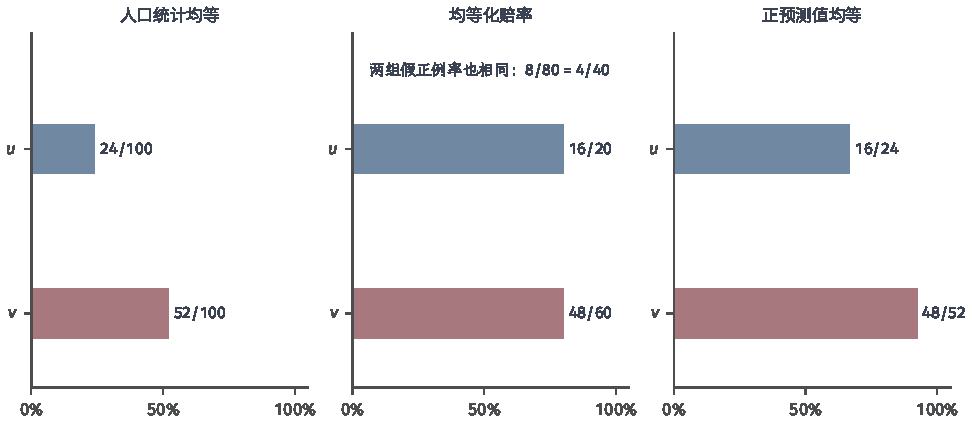
\includegraphics[width=164.600mm]{figures/03-foundations/03-trustworthiness/matplotlib/trust-fairness-incompatibility/figure.pdf}
  \caption{同一教学记录按三个分母比较：全体申请者、同资格者、已获选者。两组各100人，合格20与60，计数沿示例~\ref{ex:fairness-rates}。共同$t=0.8,f=0.1$满足均等化赔率，其他两项比例仍不同。冲突限于不同基准比例及$0<f<t<1$，$f=0$等另作分析。}
  \label{fig:trust-fairness-incompatibility}
\end{figure*}

图~\ref{fig:trust-fairness-denominators}按“资格（行）×是否获选（列）”排出两组的四项计数。读图时看每个指标的分母落在哪些格子，就能判断它保护的是全体申请者、合格者、不合格者还是已获选者。

\begin{figure*}[!htb]
  \centering
  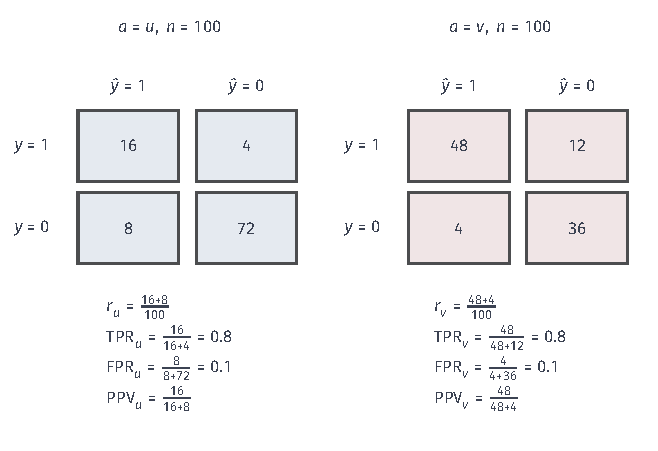
\includegraphics[width=111.404mm]{figures/03-foundations/03-trustworthiness/tikz/trust-fairness-denominators/figure.pdf}
  \caption{按资格为行、是否获选为列排列示例~\ref{ex:fairness-rates}两组计数，下方指标各取相应分母。真正例和假正例一致仍可伴随机会及预测值不同。计数未包括概率，不能检验分数校准。}
  \label{fig:trust-fairness-denominators}
\end{figure*}

混淆矩阵只记录类别计数，不含个人的概率分数，因此无法检验校准。另构造两组各10人都得到0.8分，其中合格者分别为8人和6人，则两组在0.8分上的经验合格率是0.8和0.6，第二组比分数声称的低0.2。这一发现与前面总计数的例子可以同时成立，说明相同错误率没有包含分数层面的信息。每组10人的样本量很小，总体校准是否真的失败还要估计误差。

实践中应按选定准则同时保存混淆矩阵与分数。获选/总人数、合格获选/合格人数、合格获选/获选人数分别对应机会率、真正例率和正预测值；校准则按组和分数区间比较平均预测与实际频率。条件和分母不同，同一份记录回答的是不同问题。

\paragraph{交叉群体中的分数检验}

按组校准与人口统计均等有同样的漏洞：对每个单属性组校准良好，某些交叉子群仍可能被持续高估或低估。\term{多重校准}（multicalibration）把子群细化的思路用于校准：在每个可识别子群的每个分数区间内，平均预测分数与实际事件频率之差都不超过给定容差\scite{hebertjohnson2018multicalibration}。

沿用第~\ref{sec:reliability-evaluation}节的分箱做法，令$\mathcal B$为分数区间族。太小的“子群×区间”格子里样本极少，估计完全被噪声主导，因此预先给定最小概率质量$\rho>0$，只对足够大的格子提出要求：
\[
 \mathcal A=\{(g,B)\in\mathcal G\times\mathcal B:
 \mathbb P(g(\bm{x},a)=1,S\in B)\geq\rho\}.
\]
对每个格子计算平均残差（实际标签减预测分数），要求所有格子的绝对残差都不超过容差$\varepsilon$：
\begin{equation}
 \sup_{(g,B)\in\mathcal A}
 \left|\mathbb E[y-S\mid
       g(\bm{x},a)=1,\ S\in B]\right|
 \leq\varepsilon.
 \label{eq:fairness-multicalibration}
\end{equation}
残差为正表示该格子被低估，为负表示被高估。用经验均值估计条件期望时，要对整个候选族统一给出误差范围；搜索后只确认一个格子违规，结论也仅限于该格子。多重校准不要求各组的成功率相同，与均等化赔率类准则保护的关系不同。

\subsection{相似个体的处理差异}
\label{sec:fairness-individual-comparison}

所有群体准则都有一个共同盲区：群体统计量相同，并不保护群体内部每一对条件相近的具体个人。\term{个体公平}（individual fairness）换了出发点：任务相关条件相近的人，应当得到相近的处理。难点不在“相近”这个词，而在于先要定义“在任务相关的意义上多近算相近”。任务认可的距离度量本身就是定义的一部分，需要规范依据，不能由数据自动给出。

Dwork 等用一个相似性界形式化这一要求\scite{dwork2012awareness}。把个体的完整审计状态记为$\bm z=(\bm x,a)\in\mathcal Z$；任务要决定哪些分量允许计入距离——记录属性$a$不等于允许依据它区别待遇。令$q_{\bm z}$表示状态$\bm z$得到的决策概率分布（确定性决策是其退化情形），$d$为任务认可的个体间距离，$D$为两个决策分布之间的差异度量。对所有个体对要求
\begin{equation}
 D(q_{\bm z},q_{\bm z'})\leq d(\bm z,\bm z').
 \label{eq:fairness-individual}
\end{equation}
这个不等式说的是：两人的待遇差别不能超过他们在任务上的差别。对二元录取规则取总变差距离时，两个分布只有“录取”与“不录取”两个结果，$D$就是两人录取概率之差的绝对值，于是“相近处理”成为一个可计算的量。

举个数值例子：距离只有0.05的两人，录取概率若分别是0.9和0.1，决策差0.8远大于0.05，违反界；若概率为0.60和0.63，决策差0.03小于0.05，这一对达标。这个例子同时显示了准则的规范负担：距离$d$必须有正当依据。若把历史收入纳入距离，而历史收入本身包含过去的机会不平等，就等于把既有不平等当成“合理差异”再要求系统复现。因此个体公平的结论只相对于所声明的距离成立。若采用随机化决策，该准则保护的是事前的决策概率：条件相同的两个人参加同一次抽签，仍可能一个中一个不中。

检验时先冻结距离定义和决策分布的估计方式，再搜索超限值$D(q_{\bm z},q_{\bm z'})-d(\bm z,\bm z')>0$的个体对。系统接口直接给出决策概率时，可以直接计算超限值；只能反复调用随机接口时，要用抽样估计概率并给出误差区间。在有限个体对中没找到反例，只支持“已检查范围内达标”，报告应写明搜索范围和发现的最大超限值。

群体准则与个体准则互不推出，两个构造可以说明。其一：两组各有一高一低两名申请者，第一组只选高资格者、第二组只选低资格者，两组机会率都是一半，人口统计均等满足，但同等资格者得到了相反待遇，个体准则违反。其二：各组高资格者比例不同，规则对所有人都只选高资格者；若规定同资格距离为0、异资格距离为1，式~\eqref{eq:fairness-individual}成立，但两组机会率不同，人口统计均等违反。两类准则保护的关系不同，检验要分别做。

\subsection{决策依据与影响路径}
\label{sec:fairness-counterfactual-comparison}

前面的统计准则只回答“各组结果是否相同”，无法回答“受保护属性是不是通过被禁止的路径影响了决定”。例如测验分数对某组系统偏低，是能力差异还是测验本身的偏差？回答这类问题需要说明变量之间谁影响谁，即因果模型。\term{反事实公平}（counterfactual fairness）的思路是比较“同一个人”在不同属性下的结果，而不是配对现实中的两个人：固定这个人的外生背景，通过干预改变群体属性，看决策分布是否变化\scite{kusner2017counterfactual}。

令$\bm U$、$\bm X$、$A$分别为外生背景、可观测特征和群体属性。外生背景是模型中不由其他变量决定的“起点”因素，如一个人的真实能力；事实取值记为$\bm u,\bm x,a_0$。$\hat Y\in\{0,1\}$表示是否给予机会。记号$\hat Y_{A\leftarrow v}(\bm U)$表示把属性干预为允许值$v$后，同一因果机制给出的决策。反事实公平要求：对事实分布$P_{\bm X,A}$中几乎所有的$(\bm{x},a_0)$，对每个结果值$b$和允许的干预值$v$，都有
\begin{equation}
\begin{aligned}
 &\mathbb P\bigl(\hat Y_{A\leftarrow a_0}(\bm U)=b
       \mid\bm X=\bm x,A=a_0\bigr)\\
 &\qquad=\mathbb P\bigl(\hat Y_{A\leftarrow v}(\bm U)=b
       \mid\bm X=\bm x,A=a_0\bigr).
\end{aligned}
 \label{eq:fairness-counterfactual}
\end{equation}
两边的条件都是同一个人的事实观测$\bm X=\bm x,A=a_0$，差别只在干预值：左边保持属性为$a_0$，右边改为$v$。计算分三步：先根据事实观测推断外生背景$\bm U$的可能取值；再把属性改为$v$；最后用同一套因果机制生成“属性被改变后的世界”中的特征和决策，比较两个世界的决策分布。最常见的错误是只在数据表里改一列属性、却让它的所有下游变量保持不变——属性改变后，由它导致的测验分数等后果也应按机制相应改变（因果干预的概念可参考\BookChapterRef{chap:causal-inference}{卷2《数学准备：概率、因果与决策》第3章“因果响应”}）。

用一个含测量偏差的例子说明这三步。设属性$a\in\{0,1\}$、真实能力为$u$，观测测验分数$x=u+\gamma a$，其中$\gamma a$是测验对属性$a$的系统偏差。如果任务认定$\gamma a$这条路径不应影响名额分配，那么直接用$x$作决定就保留了属性影响；在因果结构正确的前提下，改用$x-\gamma a=u$可以剔除它。代入数值：取$\gamma=2$，事实为$a=1,x=7$，第一步反推$u=7-2=5$；第二步把属性设为$a=0$；第三步按机制，同一人的测验应为$x=5+0=5$。校正分数$x-\gamma a$在两个世界都是5，决策不变。相反，保留$x=7$只改$a$的取值，就是前述“只改一列不传播”的错误。还要补两点现实限制：做这种校正，计算中确实需要使用属性$a$；因果结构或系数$\gamma$不可靠时，机械相减未必合理，而仅凭观测分布通常无法唯一识别这些机制。

并非所有任务都要求属性的影响完全为零。有些任务只禁止部分路径：允许属性通过真实能力产生的间接影响，只禁止与能力无关的直接偏好。这时要明确哪些路径允许、哪些禁止，以及各自的识别条件；统一要求“属性改后决策不变”反而可能不合适。另外，属性干预只用于机制分析，并不主张让个人去改变自己的属性；第~\ref{sec:interpretability-recourse}节讨论的可实施补救行动是另一回事。

反事实审计因此要显式声明因果图和结构方程，再按上面三步检验式~\eqref{eq:fairness-counterfactual}。机制不可识别时，应报告结论在若干合理机制下的敏感性，而不是只报一个数字。混淆矩阵不提供同一个体在不同干预世界中的对应关系，边际统计量相等不能代替反事实计算。

\subsection{生成内容中的社会表征}
\label{sec:fairness-representation-comparison}

除了名额分配，模型生成的内容本身也可能造成不公平：培训或职业建议可能刻板地描述某些人群、系统性遗漏他们的可能性，或无依据地贬低其能力，这些都不会反映在录取计数里。评价表征问题，先要规定关注哪些表达及其语境，例如“证据不足时不得用身份推断能力”，再建立可核验的标注体系。

核心方法是受控对照：构造资格、经历和请求完全相同的任务，只改变与任务无关的身份线索（如姓名所暗示的性别），比较输出在描述、推荐倾向、尊重程度和无依据断言上的差异。证据充分和证据不足的提问都要测，以防模型用一律拒答制造表面均等；还要核验文本自然性与事实正确性，结合规则筛查和人工复核评价输出。词替换实验只能证明“在这组输入上观察到行为差异”，不能证明第~\ref{sec:fairness-counterfactual-comparison}节意义上的个体反事实，因为改姓名不等于按因果机制改变一个人的属性。

生成式输出有随机性，需要重复抽样，保存各类结果的比例和波动，并在不同提示模板下检查结论是否稳定。评分者本身也可能带偏差：要用带已核实标签的样本检查评分是否与标签一致、分析常见误判类型；多人评分时报告评分者间一致性。BBQ 基准专门区分模糊语境与非模糊语境下的偏差：语境信息不足以回答时，依赖刻板印象作答就暴露了偏差；语境已给出答案时，则检查偏差是否压过了证据。它提示这类内容评价必须保留证据充分性，以及文化、语言的适用范围\scite{parrish2022bbq}。

\subsection{公平要求的声明}
\label{sec:fairness-requirements}

上述五类证据不能自动拼成“系统公平”的结论。正式判定前，先要把要求写成一份完整声明：任务是什么、覆盖哪些人群、保护什么关系、资格标准是什么、禁止哪些影响路径、优先避免哪种后果；然后确定主要准则、容差、效用和资源限制，并说明验证样本与有效期限。一个指标名称只提供了一种测量方式，本身不构成完整的公平要求。

要求还要有责任层面的依据：识别相关法律、政策和领域义务，保存受影响者、领域专家和运行方的意见及其分歧；明确由谁批准准则、容差、最低水平、资源安排和属性用途。批准理由、未解决的异议、纠正入口和复查周期都应可追溯。这套程序不能消除价值冲突，但能把三样容易混在一起的东西分开：机构的偏好、实际观测到的比例、以及已经获得认可的规范依据。

以教学系统为例：可以声明资格标签$y$独立可信，要求两组真正例率绝对差不超过0.05、且两组真正例率都不低于0.8，名额总量受预算约束，同时报告假正例率、交叉组表现和申请成本（数值均为构造标准）。这里有两种不同的约束：差距约束限制两组之间的差异，最低水平约束保护每组合格者的获选率。如果有一组低于0.8，把另一组的获选率压下来可以缩小差距，却不能让低的组达标——那只是拉平，不是改善。资源与要求冲突时，应回到责任流程重新讨论，而不是悄悄放宽条件。

属性$a$在不同环节的用途必须分别声明。训练或审计中使用$a$构造公平约束，并不自动决定部署时能否读取它，后者由责任流程规定。不同方法对属性的需求也不同：分组阈值在部署时必须识别组别；某些训练约束（如对抗去偏）得到的预测器部署时不需要属性。允许哪些用途，决定了哪些候选方法可以进入选择。

还要把意图与结果分开记录：目标层说明打算满足什么，验收层说明哪个版本、在哪个人群、什么数据和假设下有何种证据。独立检验未完成、组样本不足或因果机制不可识别时，都要作为明确限制保留；“采用了某个去偏算法”这一事实本身不能证明公平。

\subsection{判定结论的形成}
\label{sec:fairness-compatibility}

声明确定了要检验什么，形成结论时还剩两个问题：所选的几条准则能否同时满足，以及有限样本和建模假设把结论支持到什么程度。某一分支的证据通过，只给出局部结论，不能直接合成为无条件的“系统公平”。

\paragraph{准则之间的取舍}

一个系统往往要同时承担多条准则，而它们可能在数学上互相冲突。这时指标分歧不是“训练得还不够”，而是各组基准比例不同带来的结构性限制。下面由群体比例推导兼容条件，目的是说明哪些目标可以共同选择。

先解释示例~\ref{ex:fairness-rates}中“错误率相同、机会却不同”的代数原因。设第$a$组合格者比例（基准比例）为$\pi_a$、真正例率为$t_a$、假正例率为$f_a$。获选者由“合格且被选中”和“不合格却被误收”两部分组成，由全概率公式，全体机会率为
\[
 r_a=\pi_a t_a+(1-\pi_a)f_a=f_a+\pi_a(t_a-f_a).
\]
如果两组共用相同的$t,f$且$t\ne f$，$r_a$就是$\pi_a$的非常数线性函数，只要$\pi_u\ne\pi_v$，$r_u$与$r_v$必然不同。所以在两组基准比例不同时，均等化赔率（共同$t,f$）与人口统计均等（$r$相同）只能在$t=f$这种退化情形下同时成立；$t=f$意味着决策与资格无关，分类器没有区分能力。示例中$r=0.1+0.7\pi_a$，代入0.2和0.6即得0.24和0.52。

同样的比例结构还决定获选者的质量。若两组共用$t$和$f$，$\pi_a\in(0,1)$且各组正决策概率大于零，由贝叶斯公式，获选者中合格的比例为
\begin{equation}
 \mathbb P(y=1\mid\hat y=1,a)
 =\frac{t\pi_a}{t\pi_a+f(1-\pi_a)}.
 \label{eq:fairness-predictive-value}
\end{equation}
分子分母同除以$t\pi_a$，右侧变为$1/[1+(f/t)(1-\pi_a)/\pi_a]$。当$t,f>0$时，$(1-\pi_a)/\pi_a$随$\pi_a$严格递减，所以整个式子关于$\pi_a$严格递增：基准比例高的组，其获选者合格率必然更高，正预测值均等无法与共同的$t,f$同时成立（$f=0$时两组都等于1，是例外）。用示例数字验证：合格率0.2的组获选者合格率为$0.16/(0.16+0.08)\approx0.667$，合格率0.6的组为$0.48/(0.48+0.04)\approx0.923$。

第三项冲突发生在分数层面。设部署分数$S\in[0,1]$在各组内都校准，各组$0<\pi_a<1$，且$\pi_u\neq\pi_v$。记组内合格者、不合格者的平均分数为$\mu_{1,a}=\mathbb E[S\mid y=1,a]$、$\mu_{0,a}=\mathbb E[S\mid y=0,a]$。一个自然的“平衡”要求是这两个条件均值跨组相同（记为$\mu_1,\mu_0$），即合格者在各组平均得分一样、不合格者也一样。下面证明它与组内校准只能在完美预测时共存。

第一步，组内校准决定了组内平均分。由全期望公式和校准条件$\mathbb E[y\mid S,a]=S$，
\[
 \mathbb E[S\mid a]=\mathbb E\bigl[\mathbb E[y\mid S,a]\mid a\bigr]=\mathbb E[y\mid a]=\pi_a.
\]
第二步，按资格把组内平均分拆开，再用跨组共用的$\mu_1,\mu_0$，得
\[
 \pi_a=\mathbb E[S\mid a]=\pi_a\mu_1+(1-\pi_a)\mu_0.
\]
第三步，移项得$\pi_a[1-(\mu_1-\mu_0)]=\mu_0$。这对$a=u,v$都成立，两式相减得到$(\pi_u-\pi_v)[1-(\mu_1-\mu_0)]=0$；由$\pi_u\neq\pi_v$得$\mu_1-\mu_0=1$。由于$S\in[0,1]$，两个均值之差最大为1，等号只能在$\mu_1=1$、$\mu_0=0$时成立；有界随机变量均值达到端点还意味着几乎处处取该端点，即合格者几乎都得1分、不合格者几乎都得0分，预测完美。因此在预测不完美且两组基准比例不同时，组内校准与“合格者、不合格者平均分数分别跨组相等”不能同时成立。

这里没有要求各组平均分数相同；恰恰相反，组内校准已使平均分数分别等于不同的$\pi_a$。平均分数平衡也不同于式~\eqref{eq:fairness-equalized-odds}的二元错误率平衡，二者不能混用。这项不相容是 Kleinberg 等系统讨论的分数公平取舍的特例，引用其结论时要保留具体条件\scite{kleinberg2016fairness}。

冲突无法靠技术消除，只能依据已记录的规范和参与过程设定优先级。例如首要目标是避免误拒合格者时，可以以机会均等为主约束，同时公开假正例率、名额总量和正预测值的代价，让取舍可见。没有被选为优化目标的准则仍需监测报告：移出目标函数不等于它的后果消失。

\paragraph{有限样本与建模假设}
\label{sec:fairness-evidence}

所有准则规定的都是总体层面的关系，而审计只有有限样本。不同证据受不同限制：群体结论受样本量和分母大小限制，个体结论还受距离定义限制，反事实结论还受因果机制限制——后两者不会因为样本增多就自动正确。各类证据都要分别报告抽样误差和建模假设的敏感性。下面只用“两组真正例率之差”这一个群体准则，演示有限样本下怎样作出判定。

真正例率的分母是组内合格者数，假正例率的分母是组内不合格者数。交叉小组很容易出现某个分母接近零；在很多组里搜索差距，还会增加偶然碰到极端值的概率（多重比较）。若敏感属性本身是补全或推断得到的，其误差也要进入审计结论，不能当作无误的身份。

规范的流程是：在看到审计标签之前，先冻结模型、阈值、指标、容差和要比较的两组，审计数据不参与这些选择。设各组合格者分别独立同分布地来自目标人群的组内合格者分布，数量为$n_u,n_v$，真正例率估计为$\hat t_u,\hat t_v$。每个$\hat t_a$是$n_a$个取值0或1的“是否获选”指示变量的平均，Hoeffding 不等式给出$\mathbb P(|\hat t_a-t_a|>\epsilon)\leq2\exp(-2n_a\epsilon^2)$。给定$\delta\in(0,1)$，令每组的失败概率为$\delta/2$，解出$\epsilon_a=\sqrt{\log(4/\delta)/(2n_a)}$；由并集界，两组同时成立的概率至少$1-\delta$，再由三角不等式，
\[
 |(t_u-t_v)-(\hat t_u-\hat t_v)|
 \leq
 \sqrt{\frac{\log(4/\delta)}{2n_u}}
 +\sqrt{\frac{\log(4/\delta)}{2n_v}}.
\]
这个界说明：任何一组合格者少，对应根号项就大，差距的置信区间就宽。代入数字：取$\delta=0.05$，若两组各有200名合格者，每组半宽约$\sqrt{\log 80/(2\times200)}\approx0.105$，差距总半宽约0.21；若其中一组只有20名合格者，该项升到约$\sqrt{\log 80/(2\times20)}\approx0.33$，差距总半宽约0.44。此时即使观测到0.2的差距，区间仍同时覆盖0和超出容差的值，无法判定；另一组样本再多、总样本再大也补不上这个缺口。

\paragraph{达标、违反与证据不足}

把判定规则一般化：相对于预设容差，差距的可靠上界仍在容差内才支持达标；可靠下界已超出容差才支持违反；置信区间跨过容差线，结论只能是证据不足。个体、反事实和内容三类证据还要分别附上距离定义、因果机制以及受控任务与评分依据。无论哪种，“未发现违规”或“统计上不显著”都不能单独作为公平的证据。

最终报告应保留各组的实际水平（不只是差距）、所用准则、数据与模型版本，并指出未覆盖的人群和未验证的假设。判定结论确定了“哪项要求在什么情境下没有满足”；至于补采数据、重新训练还是调整流程，还要回到第~\ref{sec:fairness-causes}节的形成原因。

\section{公平性的干预}
\label{sec:fairness-intervention}

同样的机会差距，可能来自数据遗漏、资格标签错误、训练加权或部署阈值等不同环节。判定告诉我们“哪条要求没被满足”，原因分析告诉我们“问题出在哪个环节”，两者结合才能选择干预；差距数字本身并不指向某个具体算法。

下面按数据（第~\ref{sec:fairness-data-intervention}节）、训练（第~\ref{sec:fairness-learning-intervention}节）和服务决策（第~\ref{sec:fairness-decision-intervention}节）三个位置处理已声明的要求，最后（第~\ref{sec:fairness-intervention-evaluation}节）用即时效果和长期证据判断措施是否改善了处境。三类措施可以组合，但解决的是不同问题：补充了少数群体数据后，训练中错误代价不合理仍可能需要调整；训练约束通过后，申诉等待时间过长仍可能需要改流程。

图~\ref{fig:trust-fairness-intervention-stages}沿数据、训练和决策三个阶段标出干预位置。它提醒读者：某个环节的问题，未必能靠调整其他环节的指标修复（如标签偏差不能靠改阈值修复），因此每项干预都要沿完整后果链验收。

\begin{figure*}[htbp]
  \centering
  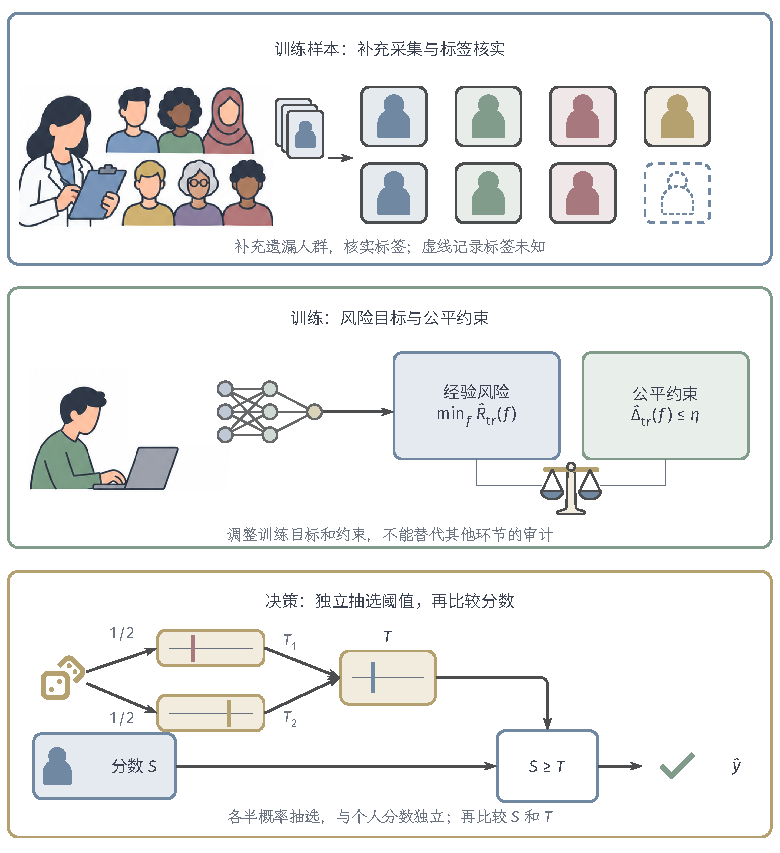
\includegraphics[width=132.000mm]{figures/03-foundations/03-trustworthiness/tikz/fairness-interventions/figure.pdf}
  \caption{从上到下依次展示数据、训练与决策阶段。数据环节补充遗漏人群并核实标签，训练环节调整风险目标及公平约束；三个位置的措施可以组合。虚线记录标签未知。决策面板画示例~\ref{ex:fairness-random-threshold}中的第一组：按预设各半概率独立抽选阈值$T$，再按分数$S$是否达到$T$产生决策$\hat y$。组内抽选独立于个人分数、其他特征及真值，第二组采用固定阈值。单环节达标未保证系统全部要求。}
  \label{fig:trust-fairness-intervention-stages}
\end{figure*}

\subsection{数据采集与质量的改进}
\label{sec:fairness-data-intervention}

确认人群遗漏后，先按任务、适用条件和交叉组定位缺口出现在哪些语言、设备、地区或资格区间，再有针对性地扩展采集渠道。新增的有效观测要与已确认的缺口对应，“两组人数相等”不是充分目标；反复复制已有类型的样本只改变训练中的出现频率，并没有增加独立个体带来的新信息。

训练时可以有意多采集困难群体，但评价时必须说明数据代表的是真实目标人口，还是为审计构造的平衡人口。改变采样比例会改变总体平均指标的含义，因此分组结果要保留，需要总体汇总时按有依据的目标人口比例加权。新的审计数据还要独立于干预方案的选择，否则反复调试后在同一批数据上验收会产生选择偏差。

测量问题要核查同一字段在不同组是否含义相同，用语言、设备的配对样本和可靠参照区分“真实能力差异”与“测量工具差异”。标签问题要复核资格定义、标注指南和争议案例，必要时重新标注。修正错误标签或不合理目标必须保留依据，不能为了让比例相同而改写真实结果。

选择性标签造成的结果缺失不能简单填成“失败”。培训只观察得到获选者的结果时，可以寻找独立的资格测验、跟踪调查或其他可靠观测；也可以在安全、合规且事先获得批准的条件下，改变后续的录取机制，让原本可能被拒的人也以正概率获选，从而留下结果证据。用统计方法修正则需要明确选择概率和识别假设（第~\ref{sec:fairness-intervention-evaluation}节给出形式）。沿用原有选择机制积累更多获选者记录，不会增加任何被拒者的信息。

采集、测量和标签方面的改变都要随数据留痕。数据集说明书记录用途、组成、采集方式和适用范围，有助于识别人群遗漏和误用，但文档本身不能替代实际补采和核验\scite{gebru2021datasheets}。

数据修好并不等于决定了分配原则。如果训练仍用总体平均目标、让多数组收益抵消小组损失，就需要继续改学习规则；如果分数本身合理但分数转行动的规则有问题，则应转到服务流程。

\subsection{训练目标与学习规则的调整}
\label{sec:fairness-learning-intervention}

当问题是模型对已有信息的使用不合理时，训练侧有三类手段，分别作用在训练的不同环节：改变不同样本错误对损失的贡献（重加权与成本敏感）；限制中间表示中保留的群体信息（公平表示、对抗去偏）；把公平准则直接写成训练约束（约束化分类）。选择哪一类取决于第~\ref{sec:fairness-causes}节诊断出的形成原因，不能因为名字里带“公平”就随意替换。

先给出约束化训练的统一形式，它说明“兼顾准确与公平”在优化上是什么意思。令训练集为$\mathcal D_{\mathrm{tr}}$、候选模型族为$\mathcal F$，由此得到经验风险$\widehat R_{\mathrm{tr}}(f)$和选定的公平差异量$\widehat\Delta_{\mathrm{tr}}(f)$（如两组真正例率的绝对差，约定为非负）。在差异不超过容限$\eta$的模型中选风险最低的：
\[
\begin{aligned}
 \min_{f\in\mathcal F}\quad &\widehat R_{\mathrm{tr}}(f)\\
 \text{subject to}\quad &\widehat\Delta_{\mathrm{tr}}(f)\leq\eta.
\end{aligned}
\]
这是训练样本上的优化问题，目标总体上的风险和差异仍须用独立数据审计。实践中常用惩罚形式$\widehat R_{\mathrm{tr}}+\lambda\widehat\Delta_{\mathrm{tr}}$（$\lambda\geq0$），因为它更容易求解；但固定$\lambda$只是加权优化，不保证差异不超过容限，要满足硬约束需要专门方法（见本节后文的归约方法）。

图~\ref{fig:trust-fairness-pareto}在构造的200人资料上同时画准确率和真正例率绝对差，用来说明怎样比较兼顾两个指标的候选。若候选甲的准确率不低于乙、差距不大于乙，且至少一项严格更好，就称甲支配乙：选甲没有任何损失。所有不被支配的候选构成当前的帕累托集合（Pareto set），真正的取舍只发生在这个集合内部。它帮助看清“提高公平要付出多少准确率、是否存在免费改进”；但换候选集、指标或评价数据都会改变这个集合，它不是普遍适用的最优边界。

\begin{figure}[htbp]
  \centering
  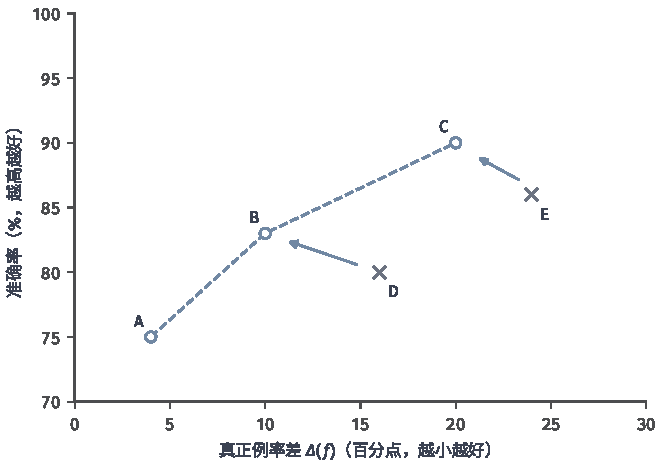
\includegraphics[width=\linewidth]{figures/03-foundations/03-trustworthiness/matplotlib/trust-fairness-pareto/figure.pdf}
  \caption{构造两组各100人、各50人合格，由五套混淆计数得到“真正例率绝对差、准确率”。A、B、C为（4个百分点，75\%）、（10个百分点，83\%）、（20个百分点，90\%），D、E为（16个百分点，80\%）、（24个百分点，86\%）。B支配D、C支配E，空心圆是当前候选中的不可支配者。虚线引导阅读，未证明中间点可实现。}
  \label{fig:trust-fairness-pareto}
\end{figure}

\paragraph{不同样本与错误的训练代价}

最简单的手段是样本重加权。小组在平均损失中的分量与人数成正比，人少就被忽略；若希望两组在经验损失中各占一半，设训练人数$n_u,n_v>0$、总数$n=n_u+n_v$，给第$a$组每个样本权重$\omega_a=n/(2n_a)$。第$a$组的权重之和是$n_a\omega_a=n/2$，于是
\[
 \frac1n\sum_{i=1}^{n}\omega_{a_i}\ell(f(\bm x_i),y_i)
 =\frac12\hat R_u(f)+\frac12\hat R_v(f),
\]
其中$\hat R_a$为组内平均损失。训练梯度按权重累积，小组样本不再仅因人少被忽略。这个方法强制的是两组对优化的影响力相等，并不强制错误率相等，也不修复有偏标签；“各占一半”这个目标本身也需要任务上的批准。改完仍要在独立数据上检查公平量。

\paragraph{表示中的信息依赖}

第二类手段针对表示层。多个下游任务复用同一个特征表示时，逐条修改每个决策规则很难控制表示中共同泄露的群体信息，这时可以直接约束表示本身。代价是：去掉群体信息的同时，也可能丢掉与之重叠的任务信号，因此要同时检验各下游任务的效用和公平结果。Zemel 等提出的学习公平表示（learning fair representations）把样本软分配到若干原型，同时优化重构误差、预测能力和组间原型分配的差异；它约束的是变换后的编码，而不是简单删除群体字段\scite{zemel2013fairrepresentations}。

记样本分配到第$k$个原型的概率为$q_k(\bm{x})$，第$a$组的平均分配为$\bar q_{k,a}$，组间差异用$\sum_k|\bar q_{k,u}-\bar q_{k,v}|$惩罚。这个惩罚与人口统计均等有一条有条件的继承关系。若先按概率向量$(q_1(\bm{x}),\ldots,q_K(\bm{x}))$抽取一个原型索引$K^*$，之后的决策只依赖$K^*$，则由全概率公式
\[
 \mathbb P(\hat y=1\mid a)=\sum_k\bar q_{k,a}\,\mathbb P(\hat y=1\mid K^*=k),
\]
右侧第二个因子不依赖组别；两组平均分配完全相同时，两组正决策率也相同。继承的条件很严格：经验分配只是近似相同，或者把整个软向量交给任意下游预测器，都不保证该结论，下游用法一改就要重新检验。这个论证也没有条件化资格标签；要继承机会均等，还须检查合格者内部的原型分布是否跨组相同。

训练时原型、软分配和下游预测器共同调整：重构项防止表示丢掉全部信息，预测项保留任务区分力，分配惩罚减少指定的组间差别，三者权重控制取舍。由于继承条件脆弱，独立数据上要分别测效用、群体可预测性和最终决策，惩罚项下降不能证明下游公平。

限制表示信息的另一种思路，是训练一个辅助预测器专门从表示或输出中挖掘残留的群体信息。\term{对抗去偏}（adversarial debiasing）让任务模型与这个“对手”竞争：任务模型既要做好任务，又要让对手猜不出属性；对手则努力猜准。Zhang 等把该思想用于减少特定差距，其效果取决于对手能看到什么、能力有多强\scite{zhang2018debiasing}。

令任务模型为$h_{\bm{\theta}}$、属性预测器为$d_{\bm{\phi}}$，相应经验损失为$L_{\mathrm{task}},L_{\mathrm{group}}$，取舍系数$\lambda\geq0$，竞争目标写为
\[
 \min_{\bm{\theta}}\max_{\bm{\phi}}
 \left\{L_{\mathrm{task}}(\bm{\theta})
       -\lambda L_{\mathrm{group}}(\bm{\theta},\bm{\phi})\right\}.
\]
对$\bm\phi$取最大等价于让对手最小化自己的群体损失；对$\bm\theta$取最小则同时压低任务损失、抬高对手的群体损失。实现时交替优化：固定任务模型训练对手猜属性，再固定对手更新任务模型。部署时通常只保留任务模型。

这个方法的边界要认清。对手猜不出属性，减少的只是“在给定函数类、样本和优化精度下可检测到的依赖”；对手没有胜过基准，并不证明属性独立，也不排除更强的攻击者，所以验收时宜另训一个独立的攻击者检验。若目标是均等化赔率，需要控制的是给定标签后的剩余依赖，可按标签分别训练对手。竞争训练也可能不稳定；任务信号与属性信息高度重叠时，取舍依然存在。

\paragraph{公平约束下的分类学习}

表示约束间接地影响公平，第三类手段则把已知准则直接写成约束。许多群体准则都可以写成条件矩约束，即“指定群体和标签下，某个指示变量的平均值应满足什么”。例如真正例率差约束可拆成两个有方向的不等式$\hat t_u-\hat t_v\leq\eta$和$\hat t_v-\hat t_u\leq\eta$，其中每个$\hat t_a$就是该组合格者上“是否获选”指示变量的均值。Agarwal 等把这种约束问题归约为\term{成本敏感分类}（cost-sensitive classification），即每个样本每种错误代价可以不同的分类：通过调整代价，反复调用现成的成本敏感学习器，在保留原模型形式的同时满足约束\scite{agarwal2018fairreductions}。

记有限约束集合为$\mathcal J$，第$j$条带方向的经验差异为$\hat g_j(f)$、容限为$\eta_j$。部署时允许按某个分布$Q$从$\mathcal F$中随机抽取分类规则，这样期望风险和期望差异都是$Q$的线性函数。问题的拉格朗日形式为
\begin{equation}
\begin{aligned}
 &\min_{\substack{Q:\ \operatorname{supp}(Q)\subseteq\mathcal F}}
 \sup_{\bm{\lambda}\in\mathbb R_+^{|\mathcal J|}}
 \left\{\mathbb E_{f\sim Q}[\widehat R_{\mathrm{tr}}(f)]\right.\\
 &\qquad\left.+
 \sum_{j\in\mathcal J}\lambda_j
 \bigl(\mathbb E_{f\sim Q}[\hat g_j(f)]-\eta_j\bigr)
 \right\}.
\end{aligned}
 \label{eq:fairness-reduction}
\end{equation}
它的作用机制可以直接读出：乘子$\lambda_j$可取任意非负值，只要第$j$项的平均差异超过容限，括号内的项为正，增大$\lambda_j$就使上确界趋于无穷；若满足约束，该项非正，最优的$\lambda_j$取0。所以只有满足全部约束的混合分类器，目标值才有限，且等于其风险。训练中乘子的实际含义就是“为违反该准则的错误增加代价”。允许混合还有一个作用：多个确定性分类器的随机混合可以实现单一确定规则达不到的中间错误率。实际算法会限制乘子范围和停止精度，公式只说明约束如何起作用。

代价反馈可以追踪到“哪组的哪种错误”：某组真正例率过低，就提高该组合格者被误拒的代价；调整后若假正例率超过上限，就提高该组不合格者被误收的代价。算法交替进行：给定乘子，训练一个成本敏感分类器；计算各约束的违规量，增大超限项的乘子；用更新后的代价重新训练，直到停止。要保存每一轮候选和最终的混合权重，不能只挑其中准确率最高的一轮。它与对抗去偏的优化形式相似，但反馈对象不同：这里反馈的是公平准则的违规量，对抗去偏反馈的是属性可预测性。

归约方法的保证依赖候选族的表达能力、成本敏感学习器的拟合能力和求解误差；经验上达标仍须独立总体审计。属性用途上要分清：技术上属性可以只在训练时用于构造约束，部署模型是否读取属性由所选模型与接口决定；规范上，属性在训练、审计、部署中的每一种用途都要分别获得许可。需要在使用时识别组别的分组阈值后处理，与只在训练阶段使用属性的方案属于不同的合规情形。

交叉组数量很多时，可以交替进行学习与审计：每轮搜索当前加权违规最高的子群，把第~\ref{sec:fairness-group-comparison}节审计所用的参照人群、质量定义和差异度量原样转成下一轮训练约束。改一个交叠组可能影响其他组，停止时要检查约定的整个子群族并用独立数据验证。

个体公平和反事实公平也可以进入训练：个体要求可按认可距离惩罚决策差超限，再用未参与优化的个体对检验；反事实要求则按认可的因果结构构造不受禁止路径影响的依据，或约束干预世界之间的决策一致。前面的测验校正$x-\gamma a$只在因果结构成立时有效，优化出的世界一致性修复不了不可靠的机制。这两类要求都不能用总体比例均等代替。

\subsection{决策规则与服务流程的调整}
\label{sec:fairness-decision-intervention}

如果不具备重新训练模型的条件，仍可以在模型之外修改两个对象：分数失准时修正分数；机会分配或错误率不满足要求时，修改把分数转成行动的规则。两者会相互影响（改分数会改变阈值的效果），各自是否达标要分别检验。

针对式~\eqref{eq:fairness-multicalibration}发现的偏差，可以按“组×分数区间”的平均残差校正分数，并继续检查交叠子群；正式方法还会控制校正步长、搜索范围和泛化误差。校正后要重新做校准；下游固定阈值产生的获选名单也可能改变，名额分配量要重新计算。

保留原分数、只改决策规则时，ROC 平面提供了几何图像。每个确定性阈值对应 ROC 平面上的一个点，横坐标是该阈值下的假正例率，纵坐标是真正例率；一个组的所有候选阈值构成该组的可达点集。如果以预先设定的概率为每个人随机抽取一个阈值，且抽取独立于该人的分数、其他特征和标签，那么期望错误率就是相应 ROC 点按这些概率的加权平均（凸组合）。于是每组的可达区域扩大为这些点的凸包，Hardt 等在各组可达区域的交集中选取共同错误率，以满足均等化赔率。

\begin{example}[随机化如何补出共同错误率]
\label{ex:fairness-random-threshold}
在独立验证结果上，第一组两个阈值对应的（假正例率，真正例率）为$(0.1,0.5)$和$(0.3,0.9)$，第二组一个阈值为$(0.2,0.7)$。第一组的两个确定性阈值都达不到第二组的点。让第一组每个人按各半的预设概率独立选择两个阈值（选择独立于分数、其他特征和标签），第一组的期望点为$0.5\times(0.1,0.5)+0.5\times(0.3,0.9)=(0.2,0.7)$，与第二组相同，均等化赔率在期望意义下满足。一次实际抽签得到的样本率仍会波动；部署时还要验证目标分布支持这些错误率，并估计相应误差。
\end{example}

后处理的代价要说清。交集点的真正例率可能低于最低要求，假正例率可能超过上限，整体效用也可能下降；错误率均等有时是靠压低原本较好组的获选水平实现的（“向低处看齐”）。后处理不能增加原排序中没有的信息；按组别随机给阈值，还可能让条件相近的个体仅因组别不同得到不同机会，因此不保证个体公平。它的好处是分数固定时取舍可以精确计算，限制是表示和排序都已固定。是否采用仍须符合属性用途规定、资源约束和实际后果。

服务流程的干预还包括复核渠道、补充材料、错误纠正，以及多语言和多种提交方式的支持，这些都要记录标准和时延。转人工不是公平的自动证明：要分别检查各组的转交比例、等待时间和最终结果；大量请求转给人工却长期得不到处理，自动部分的错误率即使下降，也不能说明服务更公平。

对生成式建议，可在服务规则中限定所需证据、应主动询问的信息和复核时的表达方式，再用第~\ref{sec:fairness-representation-comparison}节的受控身份任务验收；训练侧也可使用核实过的对照数据和反馈持续修正。“已经使用去偏数据训练”不是生成内容达标的证据。

\subsection{干预效果与持续调整}
\label{sec:fairness-intervention-evaluation}
\label{sec:fairness-long-term}

无论干预发生在数据、训练还是服务环节，都要回到同一份公平要求上验收，不能各环节用各自的指标自证。即时比较评价当下的收益；长期跟踪检查数据和系统状态改变之后要求是否仍然成立，再结合后续结果决定保留、调整或撤回措施。

\paragraph{即时效果与负担转移}

即时对照要固定任务、群体、标签和准则，在没有参与方案选择的同一批资料上比较干预前后的规则。报告应保存修改前后的效用和各组指标、二者差值，以及水平和差值各自的不确定区间；若另有预设目标，同时记录目标值与是否达标。为什么必须记录水平而不能只报差距？差距从0.2降到零有两种完全不同的方式：较低组的真正例率从0.6升到0.8，处境真实改善；或较高组从0.8降到0.6，向低处看齐。只有同时记录两组修改前后的真正例率、假正例率和获选名额，才能判断合格者的机会是否改善；还要检查负担是否被转移到其他人或其他环节，如等待时间、材料要求。

模型把请求转交人工时，要按组报告第~\ref{sec:reliability-evaluation}节的处理比例和接受风险，并计入等待时间、人工成本和最终结果。这里的“服务覆盖”指请求实际获得处理的比例，与第~\ref{chap:trust-reliability}章中预测集合覆盖真实标签是不同概念。

报告结构上，主要标准由公平要求确定，其他指标用于揭示代价；在多个指标中反复挑选最有利的一个，只会显示局部收益。样本不足时如实报告不确定性，“差异不显著”不等于不公平已经消失。

\paragraph{选择性标签与后续结果}

长期评估的难点在于干预会改变比较条件本身：曝光增加会产生更多点击和行为数据，参加培训又会真实改变未来的能力和资格。因此静态指标通过之后，仍要追踪机会、能力与负担的动态变化。

其中一项具体任务，是估计“如果某群人获得培训，平均会有什么结果”，而结果只在获选者身上观察得到。若直接用获选者的平均结果，答案会偏向原本就更容易获选的人。为避免把培训后的结果误当成获选前的资格，记培训后的结果为$z$，是否获得机会为$r\in\{0,1\}$，获选后的潜在结果为$z(1)$（假如此人获选会得到的结果，无论他实际是否获选），选择概率（倾向）为$e(\bm{x},a)=\mathbb P(r=1\mid\bm{x},a)$。需要三个条件：在所考察群体上$z(1)$可积；给定特征和属性后，$r$与$z(1)$独立（条件可交换性，即同特征的人是否获选与其潜在结果无关）；$e>0$在该群体的特征分布下几乎处处成立（正概率覆盖，即每类人都有机会被选中）。获选者观测到$z=z(1)$。在这些条件下，逆概率加权给出
\begin{equation}
 \mathbb E\!\left[\frac{r z}{e(\bm{x},a)}\mid a\right]
 =\mathbb E[z(1)\mid a].
 \label{eq:fairness-selective-weight}
\end{equation}
$r=0$时乘积为零，所以无需观测未获选者的$z$。推导分两步：由于$rz=rz(1)$，先固定$(\bm x,a)$，用条件独立性得$\mathbb E[rz(1)\mid\bm x,a]=\mathbb E[r\mid\bm x,a]\,\mathbb E[z(1)\mid\bm x,a]=e(\bm x,a)\,\mathbb E[z(1)\mid\bm x,a]$，除以$e$后消去选择概率；再在组内对$\bm x$求平均，即得右侧。直观上，获选概率为$e$的那类人在获选者中只出现了应有比例的$e$倍，乘上$1/e$就把他们的权重补回来。

这些假设很脆弱。如果原获选决策使用了未记录的信息（如面试印象），给定$(\bm{x},a)$后该信息仍可能同时影响$r$和$z(1)$，条件可交换性被破坏；若某类人从未获选，正概率条件不成立，其结果在数学上无法恢复，只能另取证据；$e$很小时$1/e$很大，还会放大估计方差。Lakkaraju 等利用不同决策者（如不同审批官）选择倾向的差异来研究选择性标签下的评价，说明验证用的标签可能本身就是被待评价决策生产出来的\scite{lakkaraju2017selective}；决策者差异要能充当依据，也需要一组比较假设，不能直接当作随机实验。

干预的长期后果还取决于决策之后个体状态怎样演化。Liu 等的《Delayed Impact of Fair Machine Learning》用决策后的状态演化模型指出：在其假设下，静态公平约束既可能帮助、也可能损害被保护组，方向由新增获选者的构成、状态变化机制和原分布共同决定\scite{liu2018delayedimpact}。

用一个构造的机制例说明“多给机会未必改善状态”。设获得机会后成功使状态增加1、失败使状态减少2，成功概率为$p$，则新增一名参与者的期望状态变化为$p\cdot1+(1-p)\cdot(-2)=3p-2$。它在$p>2/3$时为正；当$p=0.5$时为$-0.5$：把机会扩展给成功率不足2/3的人，平均反而拉低其状态。这不是培训实测数据。在“其他人状态不变”的模型里，只有新增获选者的期望净收益为正时，群体平均状态才会提升，要让每个人都改善还需更强条件。反过来，费用补助、课程改进或降低失败代价都会改变这个算式中的数，这说明长期干预要作用于机制，而不能只调比例。

长期运行中出现新差异时，应回到数据、测量和干预副作用重新定位原因，再依据声明的标准和新证据调整；机制已经改变后继续加大原来的差距惩罚，未必改对地方。

\Needspace{8\baselineskip}
\section{本章小结}
\label{sec:fairness-summary}

回到开篇的问题：一个准确的模型是否公平地分配了培训名额？本章的回答是，先要给出“哪些差异合理”的规范依据，再分别检查五类对象——机会与负担、预测错误与分数含义、相似个体的待遇、属性的影响路径、生成内容中的社会表征。统计、距离、因果和内容证据各有适用条件；当各组基准比例不同时，均等化赔率、人口统计均等、正预测值均等和组内校准之间存在可以证明的冲突，只能按规范设定优先级。结论必须限定在具体任务、人群和证据之内，并区分达标、违反与证据不足。

不满足要求时，应按形成原因在数据、训练和服务流程中选择措施：补充遗漏人群的观测、修正测量与标签、调整训练代价或约束、改变分数转行动的规则和申诉服务。这些措施可以组合，却不能互相替代。验收时要保存各组原有水平、实际收益和后续变化，避免通过压低服务水平或转移负担制造表面的比例一致；选择性标签和延迟影响还提醒我们，长期后果取决于识别假设和状态演化机制。下一章把视野扩展到一般目标与行为边界；审计中采集群体属性本身，还要受到第~\ref{chap:trust-privacy}章信息保护要求的限制。

\paragraph{扩展阅读}

机会均等后处理与个体公平分别保护标签条件率和任务相似性，对照Hardt等与Dwork等可辨认各自对象、冲突及不互推关系\scite{hardt2016opportunity,dwork2012awareness}。

反事实公平与延迟影响分别依赖因果机制和后续状态模型，Kusner等与Liu等的分析可帮助区分经验率、允许路径与长期后果；结论都需保留建模假设\scite{kusner2017counterfactual,liu2018delayedimpact}。
